\documentclass{standalone}
%outline around text
\usepackage[outline]{contour}
\contourlength{1.3pt}

%tikz
\usepackage{tikz}
\usetikzlibrary{knots, cd, calc}

\begin{document}


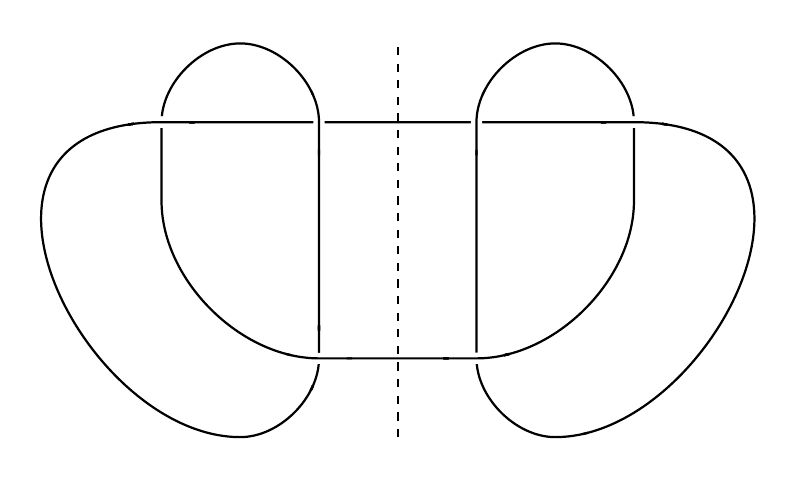
\begin{tikzpicture}
\clip (-4.7, -0.2) rectangle (4.7, 5.2);
\begin{knot}[clip width = 5, consider self intersections = true, 
ignore endpoint intersections=false,
%draft mode = crossings,
flip crossing/.list = {4, 15, 9}
]
\strand[thick] (2, 0) .. controls +(2, 0) and +(3, 0) ..
	(3, 4) --
	(-3, 4) .. controls +(-3, 0) and +(-2, 0) ..
	(-2, 0) .. controls +(0.5, 0) and +(0, -0.5) ..
	(-1, 1) -- 
	(-1, 4) .. controls +(0, 0.5) and +(0.5, 0) ..
	(-2, 5) .. controls +(-0.5, 0) and +(0, 0.5) ..
	(-3, 4) --
	(-3, 3) .. controls +(0, -1) and +(-1, 0) ..
	(-1, 1) -- 
	(1, 1) .. controls +(1, 0) and +(0, -1) ..
	(3, 3) --
	(3, 4) .. controls +(0, 0.5) and +(0.5, 0) ..
	(2, 5) .. controls +(-0.5, 0) and +(0, 0.5) ..
	(1, 4) -- 
	(1, 1) .. controls +(0, -0.5) and +(-0.5, 0) ..
	(2, 0);
\end{knot}
\draw[thick, dashed] (0, 0) -- (0, 5);
\end{tikzpicture}

\end{document}